\begin{frame}
  \frametitle{Actions(Scenarios)}

  \begin{columns}
    \column{0.5\textwidth}
    \begin{figure}[!ht]
      \centering
      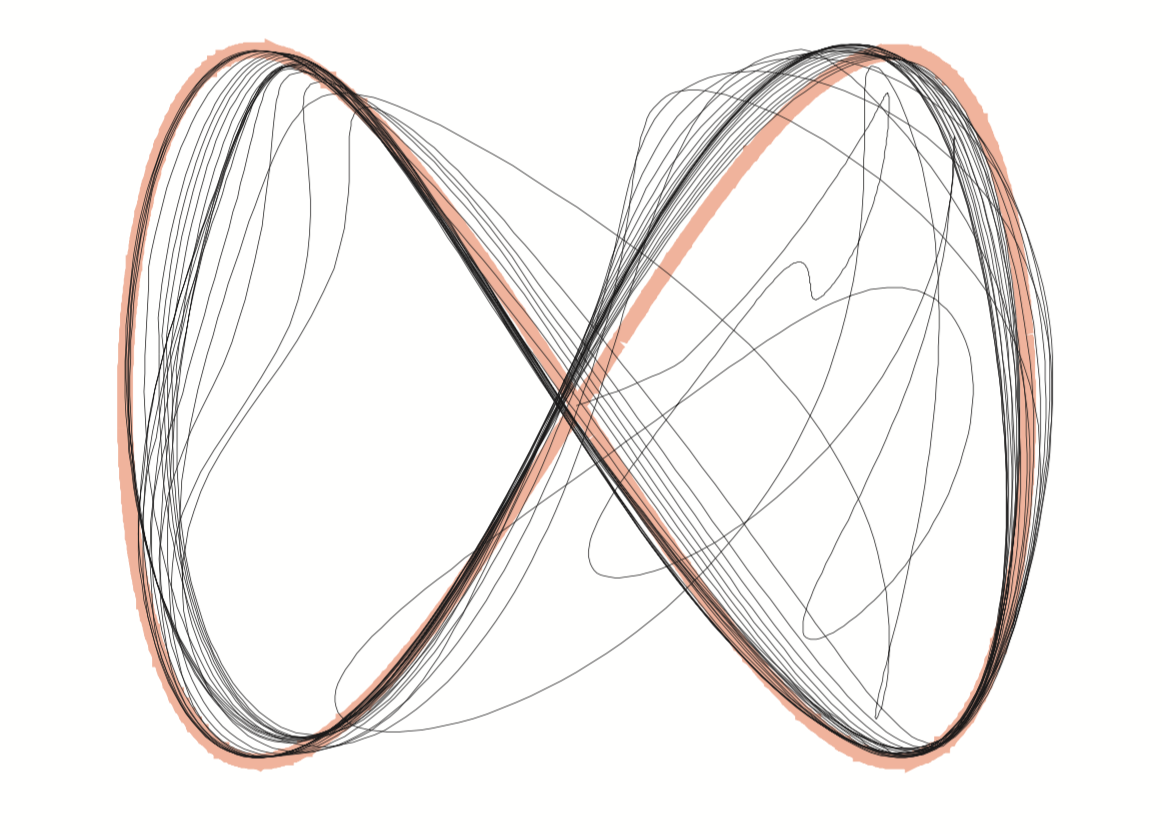
\includegraphics[width=6cm]{scene.png}
    \end{figure}

    \column{0.5\textwidth}
    \metroset{block=fill}
    \begin{block}{Natural Gesture of a Robot}
      \begin{itemize}
      \item[] Unpredictability
      \item[] Robustness
      \item[] Gesture when reaching the end effector
      \end{itemize}
    \end{block}

    \begin{block}{Learning Method}
      \begin{itemize}
      \item[] Monte Carlo(policy search)
      \item[] Dynamic Programming(value function)
      \item[] Neural Network
      \end{itemize}
    \end{block}


  \end{columns}
\end{frame}

\begin{frame}
  \frametitle{Model}
  \only<1>{
    \begin{figure}[!ht]
      \centering
      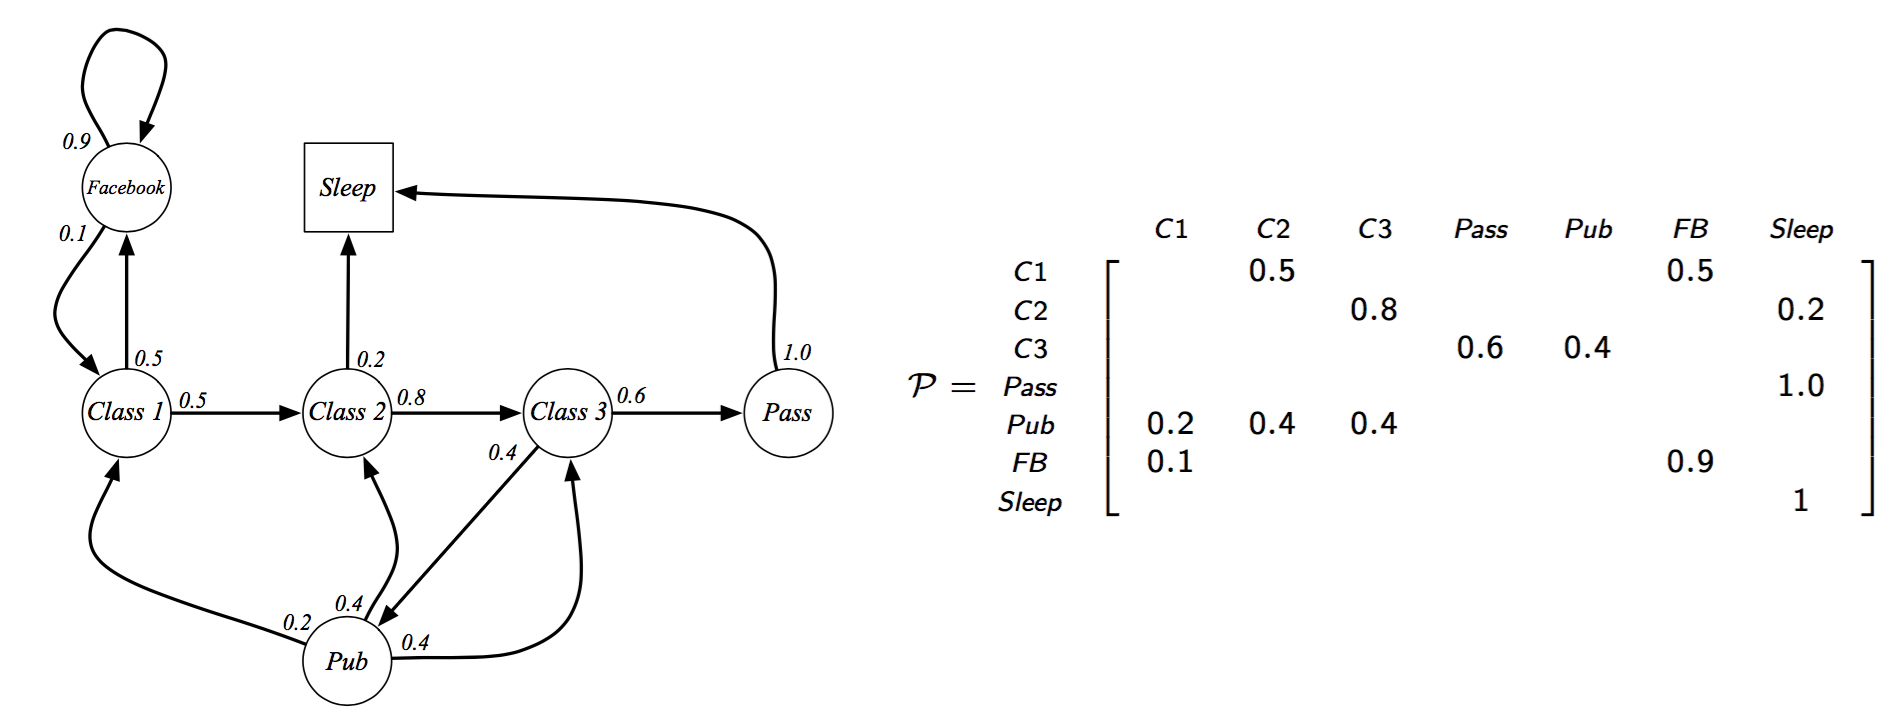
\includegraphics[width=11cm]{mdp.png}
    \end{figure}
  }
  \only<2>{
    \begin{block}{Definitions}
      \begin{itemize}
      \item[] $\pi$ ~ Policy: mapping from states to actions
      \item[] $S$ ~ A set of States
      \item[] $A$ ~ A set of Actions
      \item[] $R$ ~ Reward Function
      \item[] $P$ ~ State transition function
      \item[] $v(s)$ ~ State Value Function of a MRP
      \item[] $\gamma$ ~ Discount Function, $\gamma \in [0, 1]$
      \end{itemize}
    \end{block}
  }
  \only<3>{
    \begin{figure}[!ht]
      \centering
      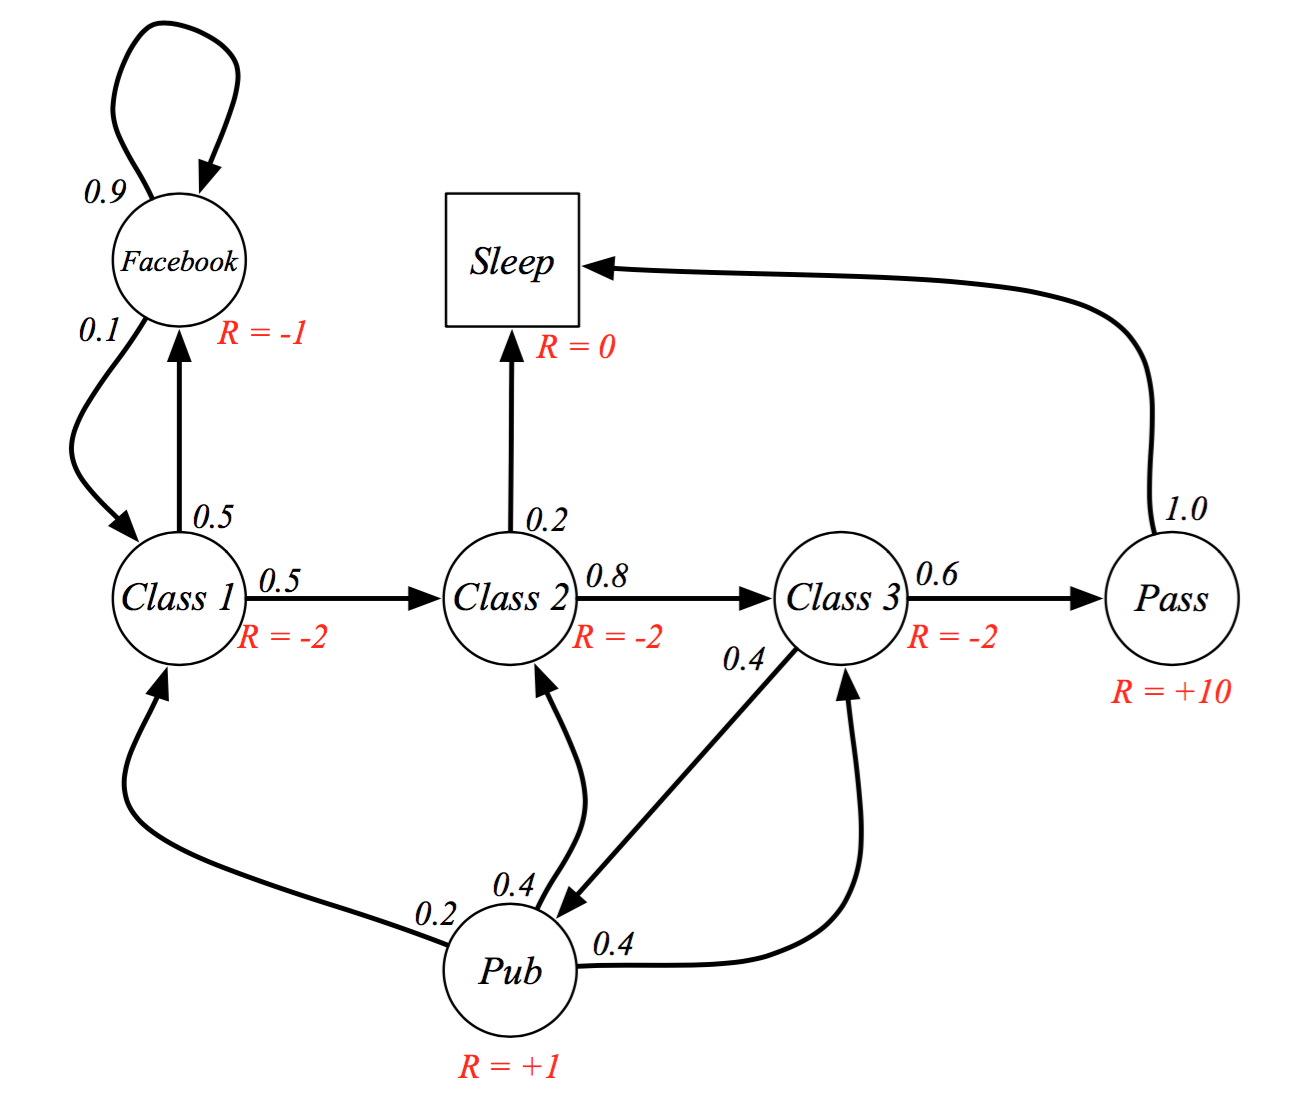
\includegraphics[width=9cm]{reward.png}
    \end{figure}
  }
\end{frame}

\begin{frame}
  \frametitle{Learning Methods}
  \begin{block}{Goal}
    Discover an optimal policy that maximizes:
    $$J=E\{\Sigma_{h=0}^HR_h\}$$
    Where $H$ is the steps the algorithm takes
  \end{block}

  \begin{exampleblock}{Expanding}
    Expanding the above with reward settings:
    $$\max_{\pi}J(\pi) = \Sigma_{s,a}\mu^{\pi}(s)\pi(s, a)R(s, a)$$
    $$s.t. \mu^{\pi} = \Sigma_{s,a}\mu^{\pi}(s)\pi(s, a)T(s,a,s'),
    \forall s'\in S,$$
    $$1 = \Sigma_{s,a}\mu^{\pi}(s)\pi(s, a)$$
    $$\pi(s, a)\le 0, \forall s\in S, a\in A$$
    
    Where $\mu$ is the distribution of states.
  \end{exampleblock}
\end{frame}

\begin{frame}
  \frametitle{Simulation}
  \begin{block}{Environment}
    \begin{itemize}
    \item Unity
    \item UR10 Avatar
    \item Simulated Data
    \item Ikpy
    \end{itemize}
  \end{block}
\end{frame}

%%% Local Variables:
%%% mode: latex
%%% TeX-master: "demo"
%%% End:
